\documentclass[10pt,letterpaper]{article}
\usepackage[T1]{fontenc}
\usepackage{lmodern,amsmath,amssymb,graphicx,booktabs,array,longtable,xurl,titlesec}
\usepackage[margin=0.75in]{geometry}
\usepackage[hidelinks]{hyperref}
\setlength{\parindent}{0pt}
\setlength{\parskip}{0.5em}
\setlength{\tabcolsep}{3pt}
\setlength{\emergencystretch}{3em}
\titlespacing*{\subsection}{0pt}{0.7em}{0.3em}
\title{Problem-Level Reasoning Case Studies\\Baseline, Supervised Adaptation, RL, and Ablations}
\author{Tuan Minh Pham, Tri Vo, Yahor Lechanka\\Purdue University}
\date{Saved-output analysis}
\begin{document}\maketitle\section*{Scope and Reading Guide}
These are 17 deliberately selected, retrospective case studies of Qwen2.5-Math-1.5B base and its adapted policies, from the fixed 300-problem MATH-train development split, disjoint from the 512 pilot training problems. They are not MATH-500 test cases or a random sample of errors. Selection covers improvements, regressions, persistent failures, grading-sensitive changes, and correct answers with flawed explanations. No case-frequency or selected-case accuracy is a population estimate.


All 12 saved policy cohorts are complete on the same 300 problems. Before comparison, the exporter checks IDs, problem text, reference answers, prompt hashes, greedy settings, cap, and stop tokens across policies. These fields establish evaluation matching, not equality of all training conditions. Raw responses and source hashes are archived in scratch; short quotations below must exactly match them. Original correctness labels and extracted answers are retained, even when a case exposes a grading problem.


Reference reasoning is an independently written mathematical explanation, not a quotation from the dataset solution. The original dataset solution is retained in the scratch evidence export. Diagnoses are qualitative mathematical readings, not a trained verifier or formal proof certificate. Findings describe observed outputs, not internal model reasoning or a causal explanation of training.


Code, output blocks, timeout messages and diagrams inside a completion are model-generated text: the evaluation did not execute those blocks. Independent checks use separately authored arithmetic/symbolic checks, never execution of model code. A correct final answer can coexist with invalid intermediate steps; a wrong score can coexist with correct mathematics. Only explicitly discussed steps have been reviewed, not every line of every response.


GRPO and Dr. GRPO refer to the original LR1e-6/128-update arms. The LR3e-6 correctness-only arm anchors the format/length and 128-to-512 duration comparisons. KL0.01 and clip0.1 anchor to original GRPO. Original SFT uses human solutions and common evaluation stops; follow-up SFT/RFT are separate supervised controls. RFT uses filtered self-generated targets and is not an otherwise identical optimizer-only comparison. No new inference, training, or benchmark rescoring is performed.


\section*{Selected-Problem Matrix}
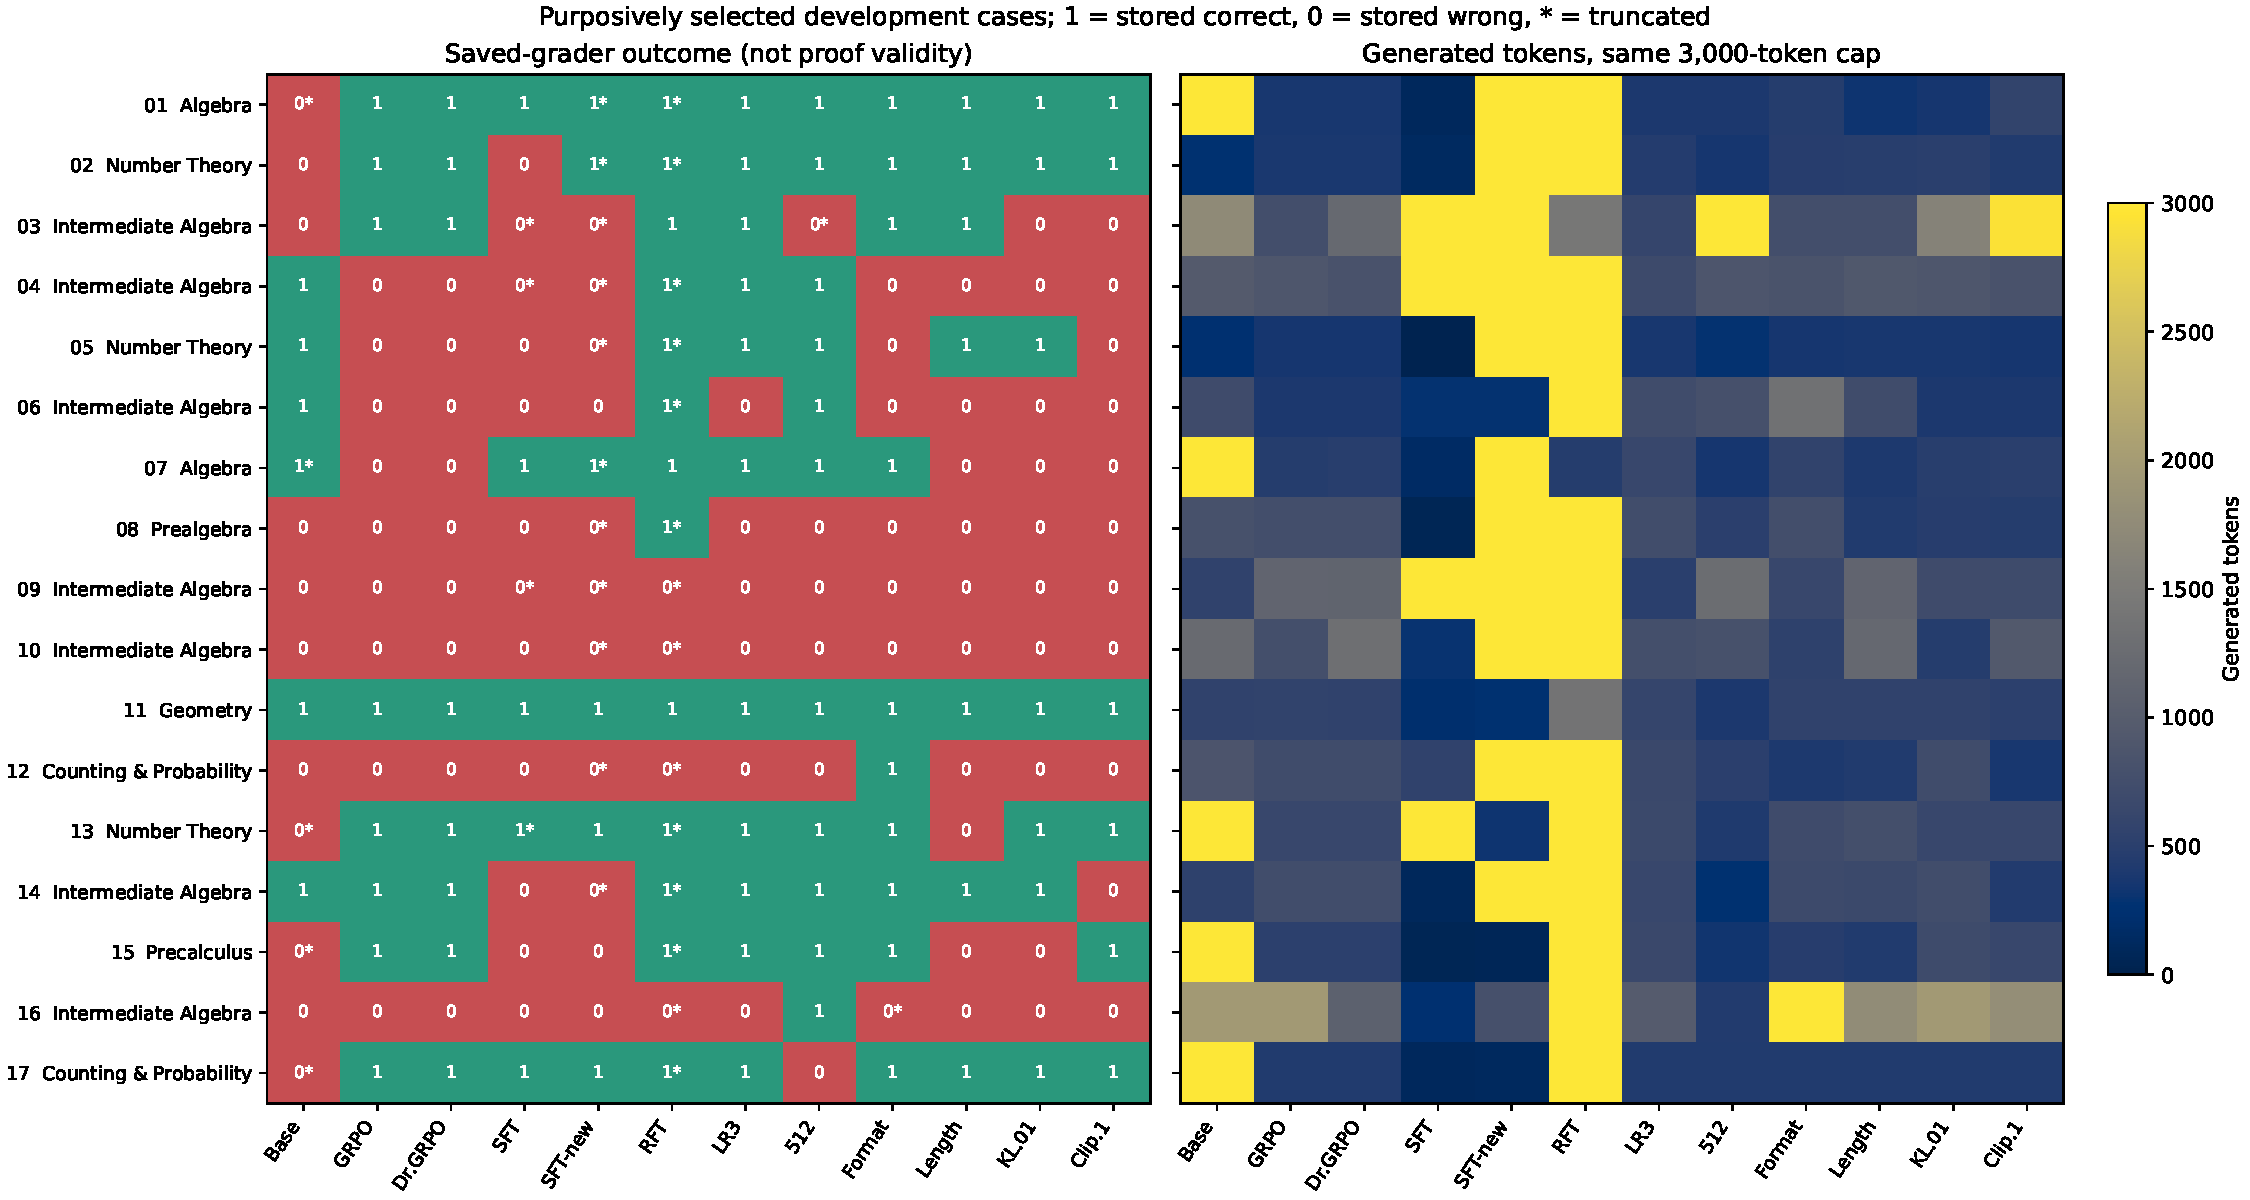
\includegraphics[width=\linewidth]{case_matrix.pdf}
\section*{Full Development Context}
Stored-grader transitions on all 300 problems, not error-type frequencies in the selected sample.
\begin{longtable}{p{0.30\linewidth}p{0.29\linewidth}rrrr}\toprule Policy & Anchor & Correct & Fixed & Broken & Truncated\\\midrule
No RL & No RL & 135 & 0 & 0 & 95\\
GRPO, LR 1e-6 & No RL & 217 & 89 & 7 & 7\\
Dr. GRPO, LR 1e-6 & No RL & 205 & 84 & 14 & 4\\
Original human-target SFT, common stops & No RL & 121 & 57 & 71 & 71\\
Follow-up human-target SFT & No RL & 131 & 65 & 69 & 209\\
Correct-solution RFT & No RL & 212 & 87 & 10 & 249\\
GRPO, LR 3e-6, 128 updates & No RL & 225 & 101 & 11 & 9\\
GRPO, LR 3e-6, 512 updates & GRPO, LR 3e-6, 128 updates & 207 & 15 & 33 & 9\\
GRPO, format bonus & GRPO, LR 3e-6, 128 updates & 222 & 17 & 20 & 7\\
GRPO, length penalty & GRPO, LR 3e-6, 128 updates & 214 & 15 & 26 & 7\\
GRPO, KL beta 0.01 & GRPO, LR 1e-6 & 213 & 13 & 17 & 10\\
GRPO, clipping 0.1 & GRPO, LR 1e-6 & 206 & 10 & 21 & 8\\
\bottomrule\end{longtable}
\clearpage\section*{Case 01: Answering the intended quadratic instead of degenerating}
Algebra, Level 3 | Completion and instruction following
\subsection*{Problem}
What value of $x$ will give the minimum value for $x^2- 10x + 24$?
\subsection*{Reference Reasoning}
$x^2-10x+24=(x-5)^2-1$, so the minimizing input is $x=5$, not the minimum function value $-1$.
\subsection*{Saved Outputs}
\small\begin{longtable}{p{0.29\linewidth}p{0.10\linewidth}p{0.35\linewidth}rr}\toprule Policy & Grade & Extracted answer & Tokens & Cap hit\\\midrule
No RL & wrong & .Highlight & 3000 & yes\\
GRPO, LR 1e-6 & correct & 5 & 366 & no\\
Original human-target SFT, common stops & correct & 5 & 113 & no\\
GRPO, LR 3e-6, 512 updates & correct & 5 & 387 & no\\
\bottomrule\end{longtable}\normalsize
\subsection*{What Changes, and What Fails}
The baseline replaces the requested minimum problem with a different maximum problem, then repeats a marker until the 3000-token limit. GRPO uses a derivative and positive second derivative; SFT completes the square and distinguishes the minimizing input from the attained value. Both approaches support the correct answer.
\subsection*{Interpretation}
This is a clear completion/instruction-following improvement, but it does not show that the baseline lacks the mathematical ability to minimize a quadratic. The observed failure never reaches a meaningful solution attempt.
\subsection*{Exact Saved-Response Excerpts}
\textbf{No RL}
\begin{quote}\small\raggedright What is the maximum value of \$y= x\textasciicircum{}2 + 10x - 24\$ in the domain \$-10\textbackslash{}leq x\textbackslash{}leq 15\$?.Highlight\end{quote}
\textbf{GRPO, LR 1e-6}
\begin{quote}\small\raggedright f\_prime = sp.diff(f, x)\end{quote}
\textbf{Original human-target SFT, common stops}
\begin{quote}\small\raggedright (x-5)\textasciicircum{}2-1\end{quote}
\clearpage\section*{Case 02: An apparent RL fix that is actually answer extraction}
Number Theory, Level 3 | Grading and answer formatting
\subsection*{Problem}
How many positive three-digit integers are divisible by both 11 and 5?
\subsection*{Reference Reasoning}
The common multiples are multiples of $55$. Their multipliers range from $2$ through $18$, giving $18-2+1=17$.
\subsection*{Saved Outputs}
\small\begin{longtable}{p{0.29\linewidth}p{0.10\linewidth}p{0.35\linewidth}rr}\toprule Policy & Grade & Extracted answer & Tokens & Cap hit\\\midrule
No RL & wrong & there are 17 positive three-digit integers that are divisible by both 11 and 5. & 258 & no\\
GRPO, LR 1e-6 & correct & 17 & 384 & no\\
Original human-target SFT, common stops & wrong & 9 & 129 & no\\
GRPO, LR 3e-6, 128 updates & correct & 17 & 452 & no\\
\bottomrule\end{longtable}\normalsize
\subsection*{What Changes, and What Fails}
The baseline identifies the correct endpoints and explicitly computes 17. Its saved extracted answer is an entire concluding sentence, and the historical grader marks it incorrect. GRPO boxes 17 and receives credit. The mathematics is already correct before training in this response.
\subsection*{Interpretation}
Count this as an extraction/formatting-sensitive score change, not a newly acquired counting strategy. Historical labels are preserved rather than silently corrected; a separate grader audit would be required to revise benchmark totals.
\subsection*{Exact Saved-Response Excerpts}
\textbf{No RL}
\begin{quote}\small\raggedright (990 - 110) / 55 + 1 = 16 + 1 = 17\end{quote}
\textbf{No RL}
\begin{quote}\small\raggedright Therefore, there are 17 positive three-digit integers that are divisible by both 11 and 5.\end{quote}
\textbf{GRPO, LR 1e-6}
\begin{quote}\small\raggedright \textbackslash{}boxed\{17\}\end{quote}
\clearpage\section*{Case 03: A genuine correction of exponent manipulation}
Intermediate Algebra, Level 4 | Algebraic reasoning improvement
\subsection*{Problem}
Simply the expression
\[\frac{(\sqrt{2} - 1)^{1 - \sqrt{3}}}{(\sqrt{2} + 1)^{1 + \sqrt{3}}},\]writing your answer as $a - b \sqrt{c},$ where $a,$ $b,$ and $c$ are positive integers, and $c$ is not divisible by the square of a prime.
\subsection*{Reference Reasoning}
Let $u=\sqrt{2}+1>0$. Since $\sqrt{2}-1=u^{-1}$, the quotient is $u^{-(1-\sqrt{3})-(1+\sqrt{3})}=u^{-2}=3-2\sqrt{2}$.
\subsection*{Saved Outputs}
\small\begin{longtable}{p{0.29\linewidth}p{0.10\linewidth}p{0.35\linewidth}rr}\toprule Policy & Grade & Extracted answer & Tokens & Cap hit\\\midrule
No RL & wrong & 1 & 1746 & no\\
GRPO, LR 1e-6 & correct & 3 - 2\textbackslash{}sqrt\{2\} & 750 & no\\
Original human-target SFT, common stops & wrong & \&= \textbackslash{}frac\{(\textbackslash{}sqrt\{3\} - \textbackslash{}sqrt\{2\})\textasciicircum{}\{\textbackslash{}sqrt\{3\}\} (\textbackslash{}sqrt\{3\} + \textbackslash{}sqrt\{ & 3000 & yes\\
GRPO, LR 3e-6, 128 updates & correct & 3 - 2\textbackslash{}sqrt\{2\} & 602 & no\\
\bottomrule\end{longtable}\normalsize
\subsection*{What Changes, and What Fails}
The baseline moves a denominator power into a positive multiplying power and then invokes an unsupported identity for irrational exponents. It finally boxes 1 despite its own preceding expression. GRPO instead changes to a common positive base, subtracts the exponents correctly, and rationalizes the denominator.
\subsection*{Interpretation}
Unlike the extraction case, both responses terminate without truncation and disagree mathematically. This is evidence of improved reasoning on this particular problem, not merely a shorter or better-formatted response.
\subsection*{Exact Saved-Response Excerpts}
\textbf{No RL}
\begin{quote}\small\raggedright are conjugates of each other\end{quote}
\textbf{No RL}
\begin{quote}\small\raggedright \textbackslash{}boxed\{1\}\end{quote}
\textbf{GRPO, LR 1e-6}
\begin{quote}\small\raggedright (\textbackslash{}sqrt\{2\} + 1)\textasciicircum{}\{-2\}\end{quote}
\clearpage\section*{Case 04: The right range strategy, followed by a sign error}
Intermediate Algebra, Level 4 | Arithmetic regression and learning-rate sensitivity
\subsection*{Problem}
Find the range of the function \[f(x) = \frac{x}{x^2-x+1},\]where $x$ can be any real number. (Give your answer in interval notation.)
\subsection*{Reference Reasoning}
The denominator is always positive. Setting $y=f(x)$ gives $yx^2-(y+1)x+y=0$ with discriminant $-3y^2+2y+1\geq0$. Hence $-1/3\leq y\leq1$; the degenerate case $y=0$ is attained at $x=0$, and the endpoints occur at $x=-1,1$.
\subsection*{Saved Outputs}
\small\begin{longtable}{p{0.29\linewidth}p{0.10\linewidth}p{0.35\linewidth}rr}\toprule Policy & Grade & Extracted answer & Tokens & Cap hit\\\midrule
No RL & correct & \textbackslash{}left[ -\textbackslash{}frac\{1\}\{3\}, 1 \textbackslash{}right] & 964 & no\\
GRPO, LR 1e-6 & wrong & \textbackslash{}left[ \textbackslash{}frac\{1\}\{3\}, 1 \textbackslash{}right] & 892 & no\\
Original human-target SFT, common stops & wrong & (-\textbackslash{}infty, 0) \textbackslash{}cup (0, 1) \textbackslash{}cup (1, \textbackslash{}infty) & 3000 & yes\\
GRPO, LR 3e-6, 128 updates & correct & \textbackslash{}left[ -\textbackslash{}frac\{1\}\{3\}, 1 \textbackslash{}right] & 680 & no\\
\bottomrule\end{longtable}\normalsize
\subsection*{What Changes, and What Fails}
The baseline obtains the correct interval. GRPO reaches the same discriminant but evaluates the negative root as positive 1/3. Its generated verification output repeats the incorrect interval. SFT introduces a different error immediately: its reciprocal rewrite is not the original function. The higher-LR GRPO response solves the inequality correctly.
\subsection*{Interpretation}
Training can preserve the overall method while damaging a local arithmetic step. The LR comparison repairs this instance, but it does not establish that increasing LR always repairs arithmetic.
\subsection*{Exact Saved-Response Excerpts}
\textbf{GRPO, LR 1e-6}
\begin{quote}\small\raggedright y = \textbackslash{}frac\{2\}\{6\} = \textbackslash{}frac\{1\}\{3\}\end{quote}
\textbf{Original human-target SFT, common stops}
\begin{quote}\small\raggedright \textbackslash{}frac\{1\}\{x - \textbackslash{}frac\{1\}\{x\} + 1\}\end{quote}
\textbf{GRPO, LR 3e-6, 128 updates}
\begin{quote}\small\raggedright y = -\textbackslash{}frac\{1\}\{3\}\end{quote}
\clearpage\section*{Case 05: Correct code logic paired with an incorrect generated output}
Number Theory, Level 4 | Code-output inconsistency
\subsection*{Problem}
Find the integer $n$, $0 \le n \le 7$, such that \[n \equiv -3737 \pmod{8}.\]
\subsection*{Reference Reasoning}
$3737=8\cdot467+1$, so $-3737\equiv-1\equiv7\pmod8$.
\subsection*{Saved Outputs}
\small\begin{longtable}{p{0.29\linewidth}p{0.10\linewidth}p{0.35\linewidth}rr}\toprule Policy & Grade & Extracted answer & Tokens & Cap hit\\\midrule
No RL & correct & 7 & 246 & no\\
GRPO, LR 1e-6 & wrong & 1 & 357 & no\\
Original human-target SFT, common stops & wrong & 1 & 31 & no\\
GRPO, LR 3e-6, 128 updates & correct & 7 & 372 & no\\
\bottomrule\end{longtable}\normalsize
\subsection*{What Changes, and What Fails}
The baseline returns 7. GRPO writes the correct procedure: calculate the positive remainder and subtract it from 8. It then claims that this code outputs 1, and boxes 1. The higher-LR response explicitly computes the positive remainder as 1 and performs the negative-residue adjustment correctly.
\subsection*{Interpretation}
This is not evidence that an external Python interpreter failed. The evaluation did not execute the displayed code. A generated output block can contradict a correct algorithm and still determine the final answer.
\subsection*{Exact Saved-Response Excerpts}
\textbf{GRPO, LR 1e-6}
\begin{quote}\small\raggedright result = 8 - remainder\_3737\end{quote}
\textbf{GRPO, LR 1e-6}
\begin{quote}\small\raggedright ```output\par 1\par ```\end{quote}
\textbf{GRPO, LR 3e-6, 128 updates}
\begin{quote}\small\raggedright -1 + 8 = 7\end{quote}
\clearpage\section*{Case 06: Functional equations: solving the right system incorrectly}
Intermediate Algebra, Level 4 | Coefficient loss and unsupported verification
\subsection*{Problem}
Suppose $f(x)$ is a rational function such that $3f\left(\dfrac{1}{x}\right)+\dfrac{2f(x)}{x}=x^2$ for $x\neq 0$.  Find $f(-2)$.
\subsection*{Reference Reasoning}
Substitute $1/x$ into the equation and eliminate $f(1/x)$. The result is $5f(x)+2x^3=3/x^2$, giving $f(-2)=(3+64)/20=67/20$.
\subsection*{Saved Outputs}
\small\begin{longtable}{p{0.29\linewidth}p{0.10\linewidth}p{0.35\linewidth}rr}\toprule Policy & Grade & Extracted answer & Tokens & Cap hit\\\midrule
No RL & correct & \textbackslash{}frac\{67\}\{20\} & 706 & no\\
GRPO, LR 1e-6 & wrong & -\textbackslash{}frac\{1\}\{2\} & 387 & no\\
Original human-target SFT, common stops & wrong & -\textbackslash{}frac\{4\}\{3\} & 291 & no\\
GRPO, LR 3e-6, 128 updates & wrong & \textbackslash{}frac\{67\}\{28\} & 724 & no\\
Correct-solution RFT & correct & \textbackslash{}frac\{67\}\{20\} & 3000 & yes\\
\bottomrule\end{longtable}\normalsize
\subsection*{What Changes, and What Fails}
The baseline derives the correct system. Original GRPO presents a plausible symbolic solver but claims its output is -1/2. Higher-LR GRPO makes an explicit algebra error: multiplying $2x$ by $-2f(x)/x$ should produce $-4f(x)$, but the response uses $-2f(x)$ and obtains a denominator of 7 rather than 5. RFT derives the correct coefficient and answer, then repeats beyond the answer to the cap.
\subsection*{Interpretation}
Higher LR does not repair every regression. RFT recovers the correct calculation here, but its correct score does not imply reliable termination or more efficient reasoning.
\subsection*{Exact Saved-Response Excerpts}
\textbf{GRPO, LR 1e-6}
\begin{quote}\small\raggedright ```output\par -1/2\par ```\end{quote}
\textbf{GRPO, LR 3e-6, 128 updates}
\begin{quote}\small\raggedright \textbackslash{}frac\{2x\textasciicircum{}3 - 2f(x)\}\{3\}\end{quote}
\textbf{Correct-solution RFT}
\begin{quote}\small\raggedright 5f(x) + 2x\textasciicircum{}3\end{quote}
\clearpage\section*{Case 07: SFT preserves an exact radical that RL rounds away}
Algebra, Level 4 | Exact-answer representation
\subsection*{Problem}
Brenda is going from $(-4,5)$ to $(5,-4)$, but she needs to stop by the origin on the way. How far does she have to travel?
\subsection*{Reference Reasoning}
Each leg of the journey has length $\sqrt{(-4)^2+5^2}=\sqrt{41}$, so the exact total is $2\sqrt{41}$.
\subsection*{Saved Outputs}
\small\begin{longtable}{p{0.29\linewidth}p{0.10\linewidth}p{0.35\linewidth}rr}\toprule Policy & Grade & Extracted answer & Tokens & Cap hit\\\midrule
No RL & correct & 2\textbackslash{}sqrt\{41\} & 3000 & yes\\
GRPO, LR 1e-6 & wrong & 12.81 & 467 & no\\
Original human-target SFT, common stops & correct & 2\textbackslash{}sqrt\{41\} & 155 & no\\
GRPO, LR 3e-6, 128 updates & correct & 2\textbackslash{}sqrt\{41\} & 634 & no\\
\bottomrule\end{longtable}\normalsize
\subsection*{What Changes, and What Fails}
The baseline and SFT use the correct two-segment distance calculation. The baseline then degenerates after its correct answer; SFT ends compactly. GRPO computes the same geometry numerically but boxes the rounded decimal 12.81. Higher-LR GRPO retains the exact radical.
\subsection*{Interpretation}
The GRPO failure is not an incorrect distance formula. It is loss of exactness under the saved grading protocol. This is also a concrete case where SFT is shorter and receives credit while original GRPO does not.
\subsection*{Exact Saved-Response Excerpts}
\textbf{GRPO, LR 1e-6}
\begin{quote}\small\raggedright \textbackslash{}boxed\{12.81\}\end{quote}
\textbf{Original human-target SFT, common stops}
\begin{quote}\small\raggedright \textbackslash{}boxed\{2\textbackslash{}sqrt\{41\}\}\end{quote}
\textbf{GRPO, LR 3e-6, 128 updates}
\begin{quote}\small\raggedright Therefore, the exact distance is:\end{quote}
\clearpage\section*{Case 08: RFT reaches the correct package count through a flawed explanation}
Prealgebra, Level 5 | Correct outcome with invalid intermediate reasoning
\subsection*{Problem}
The landlord of an apartment building needs to purchase enough digits to label all of the apartments from 100 through 125 on the first floor and 200 through 225 on the second floor. The digits can only be purchased in a package that contains one of each digit 0 through 9. How many packages must the landlord purchase?
\subsection*{Reference Reasoning}
Count digit occurrences across both floors. Digit 1 appears $26+10+3+10+3=52$ times; digit 2 appears $26+6+3+6+3=44$ times. The remaining digits occur fewer times, so 52 packages suffice and are necessary.
\subsection*{Saved Outputs}
\small\begin{longtable}{p{0.29\linewidth}p{0.10\linewidth}p{0.35\linewidth}rr}\toprule Policy & Grade & Extracted answer & Tokens & Cap hit\\\midrule
No RL & wrong & 26 & 800 & no\\
GRPO, LR 1e-6 & wrong & 26 & 752 & no\\
Original human-target SFT, common stops & wrong & 6 & 60 & no\\
Correct-solution RFT & correct & 52 & 3000 & yes\\
\bottomrule\end{longtable}\normalsize
\subsection*{What Changes, and What Fails}
The baseline and GRPO describe the correct counting algorithm but print impossible digit histograms and answer 26. RFT boxes the correct 52, yet claims the hundreds digit on the second floor is responsible for another 26 ones and also overcounts twos as 52. Its tens/units explanation is incorrect, and it repeats after the answer until truncation.
\subsection*{Interpretation}
This is a counterexample to equating final-answer reward with valid reasoning. The RFT response receives credit, but the displayed count of digit 1 is not a correct proof of that answer.
\subsection*{Exact Saved-Response Excerpts}
\textbf{No RL}
\begin{quote}\small\raggedright [6, 26, 26, 26, 26, 26, 26, 26, 26, 26]\end{quote}
\textbf{Correct-solution RFT}
\begin{quote}\small\raggedright The digit 1 appears 26 (from 100-125) + 26 (from 200-225) = 52 times.\end{quote}
\textbf{Correct-solution RFT}
\begin{quote}\small\raggedright The digit 2 appears 26 (from 100-125) + 26 (from 200-225) = 52 times.\end{quote}
\clearpage\section*{Case 09: A persistent proof gap: three integer roots force the fourth}
Intermediate Algebra, Level 5 | Unjustified existence and missing coefficient constraint
\subsection*{Problem}
The coefficients of the polynomial
\[x^4 + bx^3 + cx^2 + dx + e = 0\]are all integers.  Let $n$ be the exact number of integer roots of the polynomial, counting multiplicity.  For example, the polynomial $(x + 3)^2 (x^2 + 4x + 11) = 0$ has two integer roots counting multiplicity, because the root $-3$ is counted twice.

Enter all possible values of $n,$ separated by commas.
\subsection*{Reference Reasoning}
Three integer roots of a monic integer quartic force the fourth to be an integer by Vieta's sum formula. Thus exactly three is impossible. Examples for 0, 1, 2, and 4 integer roots are $x^4+1$, $x(x^3-2)$, $x^2(x^2+1)$, and $x^4$, respectively.
\subsection*{Saved Outputs}
\small\begin{longtable}{p{0.29\linewidth}p{0.10\linewidth}p{0.35\linewidth}rr}\toprule Policy & Grade & Extracted answer & Tokens & Cap hit\\\midrule
No RL & wrong & 0, 1, 2, 3, 4 & 554 & no\\
GRPO, LR 1e-6 & wrong & 0, 1, 2, 3, 4 & 1127 & no\\
Original human-target SFT, common stops & wrong & 4 & 3000 & yes\\
GRPO, LR 3e-6, 128 updates & wrong & 0, 1, 2, 3, 4 & 501 & no\\
GRPO, LR 3e-6, 512 updates & wrong & 0, 1, 2, 3, 4 & 1269 & no\\
\bottomrule\end{longtable}\normalsize
\subsection*{What Changes, and What Fails}
The baseline treats every count from 0 to 4 as automatically achievable. GRPO supplies contradictory examples, including a four-integer-root polynomial as evidence for exactly three. The higher-LR response uses a degree-five polynomial as its example for a quartic. The selected longer-training response remains wrong by the saved final-answer label.
\subsection*{Interpretation}
More fluent case enumeration is not a proof of existence. The reviewed traces fail to enforce the relationship between integer coefficients and the remaining root; the final-answer reward alone does not identify that missing theorem application.
\subsection*{Exact Saved-Response Excerpts}
\textbf{No RL}
\begin{quote}\small\raggedright it is possible for it to have any of these values\end{quote}
\textbf{GRPO, LR 1e-6}
\begin{quote}\small\raggedright but if we remove one root\end{quote}
\textbf{GRPO, LR 3e-6, 128 updates}
\begin{quote}\small\raggedright (x-1)\textasciicircum{}3(x\textasciicircum{}2 + 4x + 11)\end{quote}
\clearpage\section*{Case 10: Symbolic cancellation without checking invertibility}
Intermediate Algebra, Level 5 | Missing domain and nondegeneracy conditions
\subsection*{Problem}
Let
\[f(x) = \frac{2x + 3}{kx - 2}.\]Find all real numbers $k$ so that $f^{-1}(x) = f(x).$
\subsection*{Reference Reasoning}
The composition reduces to $(4+3k)x/(4+3k)$ only when $4+3k\ne0$. At $k=-4/3$ the original map is constant on its domain and not invertible. At $k=0$, $f(x)=-x-3/2$ is a valid involution. Hence all real $k$ except $-4/3$ work on the corresponding natural domains.
\subsection*{Saved Outputs}
\small\begin{longtable}{p{0.29\linewidth}p{0.10\linewidth}p{0.35\linewidth}rr}\toprule Policy & Grade & Extracted answer & Tokens & Cap hit\\\midrule
No RL & wrong & k \textbackslash{}neq 0 & 1228 & no\\
GRPO, LR 1e-6 & wrong & k \textbackslash{}in \textbackslash{}mathbb\{R\} \textbackslash{}setminus \textbackslash{}\{0\textbackslash{}\} & 762 & no\\
Original human-target SFT, common stops & wrong & -\textbackslash{}frac\{4\}\{3\} & 300 & no\\
GRPO, LR 3e-6, 128 updates & wrong & k \textbackslash{}in \textbackslash{}mathbb\{R\} \textbackslash{}setminus \textbackslash{}\{0\textbackslash{}\} & 770 & no\\
GRPO, LR 3e-6, 512 updates & wrong & 1, -1 & 798 & no\\
\bottomrule\end{longtable}\normalsize
\subsection*{What Changes, and What Fails}
The baseline and GRPO derive the useful composition but cancel the factor that carries the exceptional parameter value. They exclude k=0 instead, incorrectly treating an everywhere-defined affine map as invalid. Higher-LR GRPO repeats the wrong restriction. The selected later checkpoint is still wrong by its saved label.
\subsection*{Interpretation}
The central failure is not failure to manipulate the fraction; it is failure to track the conditions under which the manipulation and inverse exist. Longer training does not automatically repair this example.
\subsection*{Exact Saved-Response Excerpts}
\textbf{No RL}
\begin{quote}\small\raggedright \textbackslash{}frac\{(4 + 3k)x\}\{3k + 4\}\end{quote}
\textbf{GRPO, LR 1e-6}
\begin{quote}\small\raggedright the only constraint is \textbackslash{}( k \textbackslash{}neq 0 \textbackslash{})\end{quote}
\textbf{GRPO, LR 3e-6, 128 updates}
\begin{quote}\small\raggedright The denominator \textbackslash{}( kx - 2 \textbackslash{}) should not be zero for any \textbackslash{}( x \textbackslash{}), which means \textbackslash{}( k \textbackslash{}neq 0 \textbackslash{}).\end{quote}
\clearpage\section*{Case 11: All answers are correct, but the verification snippets are not}
Geometry, Level 3 | Outcome correctness versus trace validity
\subsection*{Problem}
We have a triangle $\triangle ABC$ such that $AB = AC = 8$ and $BC = 10.$ What is the length of the median $AM$?
\subsection*{Reference Reasoning}
The median to the base of an isosceles triangle is perpendicular to it. Therefore $AM^2=8^2-5^2=39$, so $AM=\sqrt{39}$.
\subsection*{Saved Outputs}
\small\begin{longtable}{p{0.29\linewidth}p{0.10\linewidth}p{0.35\linewidth}rr}\toprule Policy & Grade & Extracted answer & Tokens & Cap hit\\\midrule
No RL & correct & \textbackslash{}sqrt\{39\} & 562 & no\\
GRPO, LR 1e-6 & correct & \textbackslash{}sqrt\{39\} & 563 & no\\
Original human-target SFT, common stops & correct & \textbackslash{}sqrt\{39\} & 216 & no\\
GRPO, LR 3e-6, 128 updates & correct & \textbackslash{}sqrt\{39\} & 600 & no\\
\bottomrule\end{longtable}\normalsize
\subsection*{What Changes, and What Fails}
The baseline and GRPO give the correct Apollonius derivation, but their later Python formula yields a squared median of 51.5, not 39. The higher-LR code gives squared median 39 and is consistent. SFT's final Pythagorean argument is correct, although its generated Asymptote coordinates do not realize the stated side lengths.
\subsection*{Interpretation}
Correct final answers can coexist with incorrect auxiliary code or diagrams. Trace-level review distinguishes a valid mathematical derivation from a falsely reassuring verification block.
\subsection*{Exact Saved-Response Excerpts}
\textbf{No RL}
\begin{quote}\small\raggedright AM\_squared = (AB**2 + AC**2 - (BC/2)**2) / 2\end{quote}
\textbf{GRPO, LR 3e-6, 128 updates}
\begin{quote}\small\raggedright median\_AM\_squared = (AB**2 + AC**2 - (BC**2 / 2)) / 2\end{quote}
\textbf{Original human-target SFT, common stops}
\begin{quote}\small\raggedright AM\textasciicircum{}2 + 5\textasciicircum{}2 = 8\textasciicircum{}2\end{quote}
\clearpage\section*{Case 12: A format-reward run changes the counting method, not just the box}
Counting \& Probability, Level 5 | Reward-ablation improvement on one instance
\subsection*{Problem}
How many different positive three-digit integers can be formed using only the digits in the set $\{2, 3, 5, 5, 5, 6, 6\}$ if no digit may be used more times than it appears in the given set of available digits?
\subsection*{Reference Reasoning}
There are $4^3=64$ strings over the four distinct digits. Ten overuse digit 2, ten overuse digit 3, and one is 666. These exclusions are disjoint, giving $64-10-10-1=43$.
\subsection*{Saved Outputs}
\small\begin{longtable}{p{0.29\linewidth}p{0.10\linewidth}p{0.35\linewidth}rr}\toprule Policy & Grade & Extracted answer & Tokens & Cap hit\\\midrule
No RL & wrong & 25 & 858 & no\\
GRPO, LR 1e-6 & wrong & 102 & 718 & no\\
Original human-target SFT, common stops & wrong & 192 & 555 & no\\
GRPO, LR 3e-6, 128 updates & wrong & 30 & 661 & no\\
GRPO, format bonus & correct & 43 & 400 & no\\
\bottomrule\end{longtable}\normalsize
\subsection*{What Changes, and What Fails}
The baseline explicitly misreads the available multiplicity of digit 5 and includes forbidden strings. GRPO's position-based counting does not consistently deduplicate repeated copies. The format-bonus policy instead forms a set of permutations and returns 43; independent enumeration confirms this number.
\subsection*{Interpretation}
The changed response is mathematically better here, not merely better formatted. This does not show that the format bonus generally helps: it is a selected local improvement within a condition whose aggregate result was worse than its correctness-only anchor.
\subsection*{Exact Saved-Response Excerpts}
\textbf{No RL}
\begin{quote}\small\raggedright we can use at most one 5\end{quote}
\textbf{GRPO, format bonus}
\begin{quote}\small\raggedright unique\_permutations = set(permutations(digits, 3))\end{quote}
\textbf{GRPO, format bonus}
\begin{quote}\small\raggedright \textbackslash{}boxed\{43\}\end{quote}
\clearpage\section*{Case 13: Length shaping introduces an inadmissible divisor pattern}
Number Theory, Level 4 | Reward-ablation regression and flawed correct traces
\subsection*{Problem}
What is the smallest positive integer with exactly 14 positive divisors?
\subsection*{Reference Reasoning}
Exactly 14 divisors allows exponents 13 or the pair 6,1. The minimal candidates are $2^{13}=8192$ and $2^6\cdot3=192$, so the minimum is 192. A square-free product of three primes has 8 divisors, not 14.
\subsection*{Saved Outputs}
\small\begin{longtable}{p{0.29\linewidth}p{0.10\linewidth}p{0.35\linewidth}rr}\toprule Policy & Grade & Extracted answer & Tokens & Cap hit\\\midrule
No RL & wrong & .Highlight & 3000 & yes\\
GRPO, LR 1e-6 & correct & 192 & 634 & no\\
Original human-target SFT, common stops & correct & 192 & 3000 & yes\\
GRPO, LR 3e-6, 128 updates & correct & 192 & 676 & no\\
GRPO, length penalty & wrong & 30 & 765 & no\\
\bottomrule\end{longtable}\normalsize
\subsection*{What Changes, and What Fails}
The correctness-only higher-LR policy returns 192, but its explanation already contains extraneous divisor forms and bad candidate arithmetic. The length-penalty response admits the square-free candidate 30 and claims a generated divisor-count list makes all candidates valid. Direct counting shows 30 has only eight divisors.
\subsection*{Interpretation}
The ablation changes this final answer from right to wrong, but the anchor's reasoning was not fully sound either. The length-penalty response is actually longer here; the local error should not be attributed to shorter reasoning without evidence.
\subsection*{Exact Saved-Response Excerpts}
\textbf{GRPO, LR 3e-6, 128 updates}
\begin{quote}\small\raggedright n = p\_1\textasciicircum{}1 p\_2\textasciicircum{}1 p\_3\textasciicircum{}6\end{quote}
\textbf{GRPO, length penalty}
\begin{quote}\small\raggedright n = 2\textasciicircum{}1 \textbackslash{}times 3\textasciicircum{}1 \textbackslash{}times 5\textasciicircum{}1 = 30\end{quote}
\textbf{GRPO, length penalty}
\begin{quote}\small\raggedright [14, 14, 14, 14]\end{quote}
\clearpage\section*{Case 14: Tighter clipping changes a correct expansion into a wrong one}
Intermediate Algebra, Level 3 | Clipping-ablation regression
\subsection*{Problem}
When the graph of $y = 2x^2 - x + 7$ is shifted four units to the right, we obtain the graph of $y = ax^2 + bx + c$.  Find $a + b + c$.
\subsection*{Reference Reasoning}
A right shift gives $2(x-4)^2-(x-4)+7=2x^2-17x+43$, whose coefficient sum is 28. Equivalently evaluate the original function at $1-4=-3$.
\subsection*{Saved Outputs}
\small\begin{longtable}{p{0.29\linewidth}p{0.10\linewidth}p{0.35\linewidth}rr}\toprule Policy & Grade & Extracted answer & Tokens & Cap hit\\\midrule
No RL & correct & 28 & 528 & no\\
GRPO, LR 1e-6 & correct & 28 & 738 & no\\
Original human-target SFT, common stops & wrong & 43 & 98 & no\\
GRPO, clipping 0.1 & wrong & 26 & 443 & no\\
\bottomrule\end{longtable}\normalsize
\subsection*{What Changes, and What Fails}
The original GRPO response expands the shifted polynomial correctly. The tighter-clipping policy writes a correct symbolic substitution but claims the expansion is $2x^2-19x+43$, producing 26. This is another inconsistency between generated code and generated output.
\subsection*{Interpretation}
This illustrates a local arithmetic regression under the clipping intervention. One chosen example cannot establish a global mechanism linking tighter clipping to expansion errors.
\subsection*{Exact Saved-Response Excerpts}
\textbf{GRPO, LR 1e-6}
\begin{quote}\small\raggedright y = 2x\textasciicircum{}2 - 17x + 43\end{quote}
\textbf{GRPO, clipping 0.1}
\begin{quote}\small\raggedright shifted\_function = original\_function.subs(x, x - 4)\end{quote}
\textbf{GRPO, clipping 0.1}
\begin{quote}\small\raggedright 2*x**2 - 19*x + 43\end{quote}
\clearpage\section*{Case 15: A KL-regularized policy rejects an already valid principal value}
Precalculus, Level 3 | KL-ablation regression and incorrect range check
\subsection*{Problem}
Compute $\arccos (\cos 7).$  All functions are in radians.
\subsection*{Reference Reasoning}
$0<7-2\pi<\pi$ and cosine is $2\pi$-periodic, so the principal inverse-cosine value is $7-2\pi$.
\subsection*{Saved Outputs}
\small\begin{longtable}{p{0.29\linewidth}p{0.10\linewidth}p{0.35\linewidth}rr}\toprule Policy & Grade & Extracted answer & Tokens & Cap hit\\\midrule
No RL & wrong & Compute \$\textbackslash{}tan (\textbackslash{}arctan & 3000 & yes\\
GRPO, LR 1e-6 & correct & 7 - 2\textbackslash{}pi & 517 & no\\
Original human-target SFT, common stops & wrong & 2\textbackslash{}pi - 7 & 70 & no\\
GRPO, KL beta 0.01 & wrong & 3\textbackslash{}pi - 7 & 697 & no\\
GRPO, LR 3e-6, 512 updates & correct & 7 - 2\textbackslash{}pi & 335 & no\\
\bottomrule\end{longtable}\normalsize
\subsection*{What Changes, and What Fails}
GRPO obtains the correct principal value. The KL policy first generates that same correct value, then falsely claims it is outside the inverse-cosine range and replaces it by $3\pi-7$. The 512-update policy has the correct answer but also says 7 is less than $2\pi$, an incorrect supporting statement.
\subsection*{Interpretation}
Regularizing policy drift does not guarantee correct local range checks. Conversely, a correct longer-trained answer can still contain a contradictory explanatory sentence.
\subsection*{Exact Saved-Response Excerpts}
\textbf{GRPO, KL beta 0.01}
\begin{quote}\small\raggedright 7 - 2\textbackslash{}pi\textbackslash{}) is not within the range\end{quote}
\textbf{GRPO, KL beta 0.01}
\begin{quote}\small\raggedright \textbackslash{}boxed\{3\textbackslash{}pi - 7\}\end{quote}
\textbf{GRPO, LR 3e-6, 512 updates}
\begin{quote}\small\raggedright less than \textbackslash{}(2\textbackslash{}pi\textbackslash{}) radians\end{quote}
\clearpage\section*{Case 16: Longer RL finds a short polynomial-elimination strategy}
Intermediate Algebra, Level 4 | Training-duration improvement
\subsection*{Problem}
Let $p(x) = x^2 + bx + c,$ where $b$ and $c$ are integers.  If $p(x)$ is factor of both $x^4 + 6x^2 + 25$ and $3x^4 + 4x^ 2+ 28x + 5,$ what is $p(1)$?
\subsection*{Reference Reasoning}
If the quartics are $F$ and $G$, their common monic quadratic divides $3F-G=14(x^2-2x+5)$, so it must be $p(x)=x^2-2x+5$ and $p(1)=4$. Direct multiplication verifies that this quadratic divides both originals.
\subsection*{Saved Outputs}
\small\begin{longtable}{p{0.29\linewidth}p{0.10\linewidth}p{0.35\linewidth}rr}\toprule Policy & Grade & Extracted answer & Tokens & Cap hit\\\midrule
No RL & wrong & Reach max function call limit. & 1967 & no\\
GRPO, LR 1e-6 & wrong & Reach max function call limit. & 1967 & no\\
Original human-target SFT, common stops & wrong & -1 & 257 & no\\
GRPO, LR 3e-6, 128 updates & wrong & 8 & 973 & no\\
GRPO, LR 3e-6, 512 updates & correct & 4 & 434 & no\\
\bottomrule\end{longtable}\normalsize
\subsection*{What Changes, and What Fails}
The baseline and original GRPO repeatedly seek common roots without reaching an answer. Their text ends with a function-call-limit message, but no external tool execution is established. Higher-LR GRPO chooses the wrong sign in the quadratic factor; SFT asserts an invalid factorization. At the same LR after 512 updates, GRPO eliminates the quartic term with a linear combination and gets 4.
\subsection*{Interpretation}
This is a substantive strategy difference in matched saved greedy outputs: root hunting is replaced by degree reduction. It is an illustrative improvement, not proof that longer training consistently produces better strategies.
\subsection*{Exact Saved-Response Excerpts}
\textbf{GRPO, LR 3e-6, 128 updates}
\begin{quote}\small\raggedright The polynomial \textbackslash{}( p(x) = x\textasciicircum{}2 + 2x + 5 \textbackslash{}) is a factor of both\end{quote}
\textbf{Original human-target SFT, common stops}
\begin{quote}\small\raggedright (x\textasciicircum{}2 + 5x + 5)(x\textasciicircum{}2 - 4x + 2)\end{quote}
\textbf{GRPO, LR 3e-6, 512 updates}
\begin{quote}\small\raggedright h(x) = 14(x\textasciicircum{}2 - 2x + 5)\end{quote}
\clearpage\section*{Case 17: Longer training keeps the probability setup but loses the answer}
Counting \& Probability, Level 4 | Training-duration regression and output contamination
\subsection*{Problem}
I have a drawer with 6 forks, 6 spoons, and 6 knives in it. If I reach in and randomly remove three pieces of silverware, what is the probability that I get one fork, one spoon, and one knife?
\subsection*{Reference Reasoning}
The favorable choices number $6^3=216$, and the total is $\binom{18}{3}=816$. The probability is $216/816=9/34$, not $1/4$.
\subsection*{Saved Outputs}
\small\begin{longtable}{p{0.29\linewidth}p{0.10\linewidth}p{0.35\linewidth}rr}\toprule Policy & Grade & Extracted answer & Tokens & Cap hit\\\midrule
No RL & wrong & I have a drawer with 6 forks, 6 spoons, and 6 knives in it. If I reach in and randomly remove three pieces of silverware, what is the probability that & 3000 & yes\\
GRPO, LR 1e-6 & correct & \textbackslash{}frac\{9\}\{34\} & 431 & no\\
Original human-target SFT, common stops & correct & \textbackslash{}frac\{9\}\{34\} & 108 & no\\
GRPO, LR 3e-6, 128 updates & correct & \textbackslash{}frac\{9\}\{34\} & 431 & no\\
GRPO, LR 3e-6, 512 updates & wrong & \{(\{probability\})\} & 427 & no\\
\bottomrule\end{longtable}\normalsize
\subsection*{What Changes, and What Fails}
The 128-update higher-LR policy returns 9/34. The 512-update policy still describes the correct numerator and denominator, but its generated output and final prose replace the answer by 0.25 and 1/4. Its stored extracted answer is a literal probability placeholder from an earlier code string, adding an extraction problem to the wrong stated result.
\subsection*{Interpretation}
This is a regression in carrying a correct setup to an exact committed answer, not a failure to identify the sampling space. It counterbalances the polynomial improvement under longer training.
\subsection*{Exact Saved-Response Excerpts}
\textbf{GRPO, LR 3e-6, 128 updates}
\begin{quote}\small\raggedright \textbackslash{}boxed\{\textbackslash{}frac\{9\}\{34\}\}\end{quote}
\textbf{GRPO, LR 3e-6, 512 updates}
\begin{quote}\small\raggedright probability = favorable\_ways / total\_ways\end{quote}
\textbf{GRPO, LR 3e-6, 512 updates}
\begin{quote}\small\raggedright \textbackslash{}boxed\{\textbackslash{}frac\{1\}\{4\}\}\end{quote}
\clearpage\section*{Cross-Case Findings}
Separate three axes: mathematical reasoning, committing/extracting an answer, and stopping behavior. The 17-count case improves in score without a mathematical correction; the irrational-power case contains a genuine correction.


Improvements coexist with regressions. Higher LR repairs a sign error and residue output, but still loses a coefficient in the functional equation. Longer RL improves polynomial elimination while losing an exact probability answer.


Neither supervised adaptation nor RL universally dominates individual problems. SFT preserves an exact distance more compactly; RFT can recover a correct coefficient calculation, yet also reaches a correct count through wrong intermediate arithmetic and fails to terminate.


Final-answer reward is not trace verification. Generated code-output consistency, algebraic equivalence, exactness, domain checks and proof completeness are distinct axes for future audits. These examples motivate those checks without estimating their prevalence or changing historical benchmark totals.


\end{document}
